%======================================================================
\section{Results: BNP Paribas, 25 September 2026}\label{sec:results}
%======================================================================

All results are as of 25 September 2026. In the following month BNP's spreads widened
with French sovereign stress, the ten-year OAT yield rising above $5\%$: the senior CDS
five-year spread rose from 57 to 74bp and, in Capital IQ spreads to benchmark, the SNP from
98 to 122bp and the Tier~2 2035NC34 from 141 to 153bp by 27 October. The analysis does not
include that move.

\subsection{Capital}

CET1 was $12.97\%$ at June 2026 against a $10.43\%$ requirement: a cushion of $2.54$pp, about
EUR~20bn of losses at June 2026 risk-weighted assets of EUR~795bn. The trigger is $7.8$pp
below the ratio, about EUR~62bn of losses. Under the base-case dynamics, $20\%$ of the
simulated paths fall below the current MDA threshold at some point in the next five
years, while the trigger is almost never reached by diffusion alone. For these bonds
capital risk is first a coupon and call risk, and only then a conversion risk.

\subsection{The three bonds and the implied hazard}

Table~\ref{tab:implied} reports the implied hazards on the valuation date. Without
write-down risk the model would value the bonds at $114$--$118$, against market prices of
$94$--$98$: the mechanical features alone explain only a small part of the discount. The
implied hazards are $2.21\%$, $2.18\%$ and $2.19\%$ a year.

\begin{table}[H]
\centering
\begin{tabular}{lccc}
\toprule
 & 6.875\% NC33 & 7.20\% NC36 & 7.45\% NC35 \\
\midrule
Reset margin (bp) & 285 & 294 & 313 \\
Clean price & 94.39 & 95.25 & 97.57 \\
Bid--offer (points) & 0.26 & 0.29 & 0.15 \\
Yield-to-call spread (bp) & 279 & 274 & 269 \\
Model price with $\lambda=0$ & 114.2 & 116.9 & 117.6 \\
Implied hazard $\lambda$ (\%/yr) & 2.21 & 2.18 & 2.19 \\
Monte Carlo s.e.\ of $\lambda$ (bp) & 0.67 & 0.66 & 0.67 \\
$\Pr(\text{called at }T_1)$ & 49\% & 52\% & 58\% \\
$\Pr(\text{called at some reset})$ & 97\% & 98\% & 98\% \\
Lifetime $\Pr(\text{conversion})$ & 1.4\% & 1.6\% & 1.4\% \\
\bottomrule
\end{tabular}
\caption{Implied hazard and model outputs on 25 September 2026, base case ($\kappa=0.35$,
$\eta=100$bp, economic call rule).}
\label{tab:implied}
\end{table}

\paragraph{Cross-section.} Table~\ref{tab:eta} shows the dispersion of the three implied
hazards as a function of the spread volatility $\eta$. A deterministic refinancing spread
($\eta=0$) gives a dispersion of $8.2$bp; a stochastic one reduces it steadily, without an
interior minimum, so the cross-section does not identify $\eta$ and $100$bp is kept as an
assumption. In price terms the base-case dispersion of $2.6$bp is $0.20$--$0.22$ points, of
the size of the bid--offer: the bonds are consistent with one hazard within the precision
of the data.

\begin{table}[H]
\centering
\begin{tabular}{lccccccc}
\toprule
$\eta$ (bp) & 0 & 25 & 50 & 75 & 100 & 150 & 200\\
\midrule
Dispersion $D(\eta)$ (bp of hazard) & 8.2 & 5.8 & 4.1 & 3.0 & \textbf{2.6} & 2.0 & 1.4\\
In price points (6.875\%) & 0.63 & 0.45 & 0.32 & 0.23 & \textbf{0.20} & 0.15 & 0.11\\
\bottomrule
\end{tabular}
\caption{Cross-bond dispersion of the implied hazards on the valuation date, by
refinancing-spread volatility.}
\label{tab:eta}
\end{table}

Over the 66 weekly dates the mean dispersion is $5.9$bp with the stochastic spread and $9.3$bp
with the deterministic one. Priced at the day's common hazard, each bond's average pricing
error is within $\pm0.25$ points (range $-1.1$ to $+1.1$). Using Capital IQ benchmark yields
instead of the FRED curve, the last-date dispersion is $2.3$--$7.8$bp depending on the
benchmark assignment, so the choice of risk-free curve matters as much as the choice of
$\eta$. Figure~\ref{fig:implied} shows the implied hazards over time. The average hazard
ranged from $1.82\%$ (August 2026) to $2.69\%$ (late March 2026, when the bonds then
outstanding fell four to five points) and rose again into the September sell-off.

\begin{figure}[H]
\centering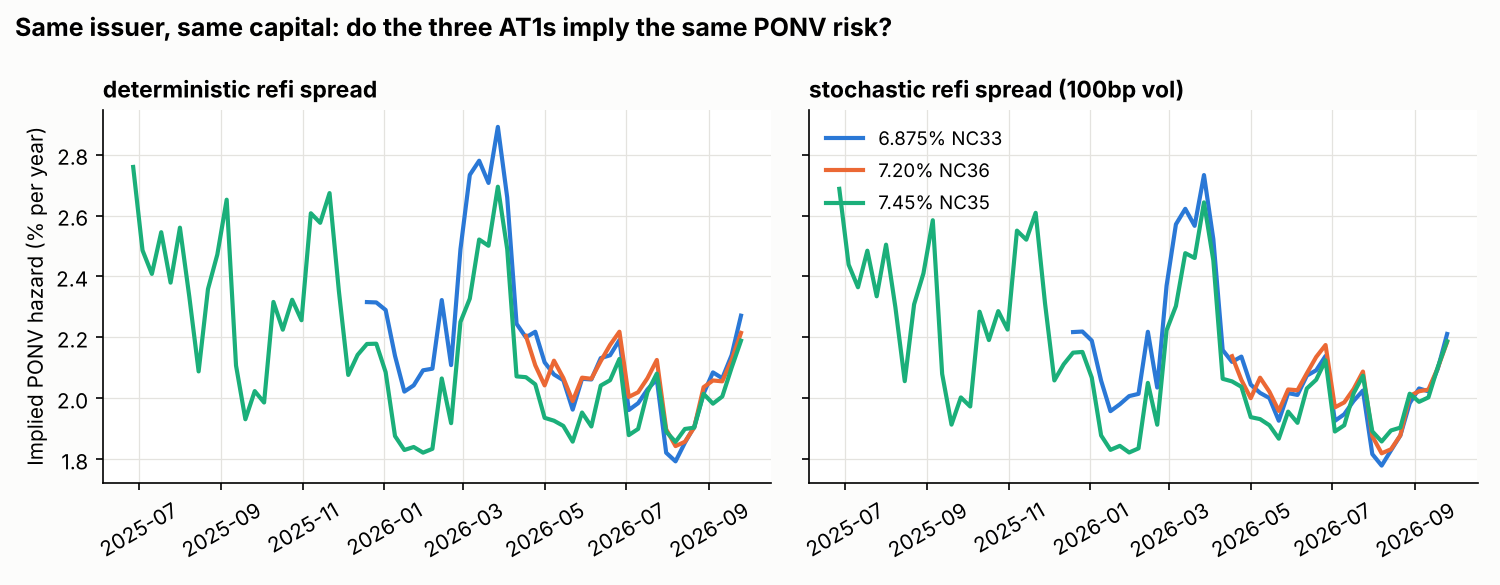
\includegraphics[width=\textwidth]{implied_ponv.png}
\caption{Implied hazard per bond, weekly, with a deterministic (left) and a stochastic
(right) refinancing spread.}
\label{fig:implied}
\end{figure}

\subsection{What BNP's Tier~2 prices}\label{sec:capstruct}

Table~\ref{tab:ladder} sets the AT1s against the rest of BNP's capital structure. Bond
hazards are implied on the same simulated state as the AT1s; CDS hazards use the credit
triangle $\lambda\approx s/(1-R)$.

\begin{table}[H]
\centering
\begin{tabular}{lcccc}
\toprule
 & Spread (bp) & Recovery & Hazard (\%/yr) & Share of AT1 hazard \\
\midrule
Senior CDS 5Y (EUR) & 57 & 40\% & 0.95 & 43\% \\
Senior CDS 7Y (EUR, 27 Sep) & 68 & 40\% & 1.13 & 52\% \\
Senior CDS 10Y (EUR, 27 Sep) & 81 & 40\% & 1.35 & 62\% \\
SNP 5.738\% 2035NC34 & 103 & 40\% & 1.63 & 74\% \\
T2 2.588\% 2035NC30 & 116 & 20\% & 1.40 & 64\% \\
\textbf{T2 5.906\% 2035NC34 (anchor)} & \textbf{144} & \textbf{20\%} & \textbf{1.72} & \textbf{78\%} \\
AT1 (average of three) & 274 & 0\% & 2.19 & 100\% \\
\bottomrule
\end{tabular}
\caption{BNP Paribas's capital structure on 25 September 2026. Bond spreads are yield to
call over the call-matched FRED Treasury.}
\label{tab:ladder}
\end{table}

The ladder is orderly: each step down the capital structure pays more. The two instruments
that share the resolution event, the Tier~2 and the SNP of the same tenor, imply nearly the
same hazard ($1.72\%$ and $1.63\%$) under the Markit recoveries. With the SNP at $40\%$, the
Tier~2 recovery that equalises the two is $R^\star=15.6\%$, close to the conventional $20\%$:
the prices of BNP's own bonds are consistent with the recovery conventions. The CDS sits
below the bonds, as one would expect of a EUR contract on senior debt compared with USD cash
bonds that carry funding and liquidity premia. The shorter Tier~2 implies a lower hazard than
the longer one, an upward-sloping term structure that Section~\ref{sec:robust} exploits.

With the Tier~2 2035NC34 as anchor,
\begin{equation}
  \lambda = 2.19\% = \underbrace{1.72\%}_{\lres:\ \text{priced in Tier~2}}
  + \underbrace{0.47\%}_{\lspec:\ \text{AT1-specific}} .
\end{equation}
By Proposition~\ref{prop:clocks}, $78\%$ of the AT1's write-down risk, in risk-neutral
terms, is compensation that BNP's Tier~2 also earns; the remaining $22\%$ is what the market
charges for being an AT1 rather than a Tier~2. Over the 66 weekly dates the Tier~2 share
ranges from $66\%$ to $80\%$, with a mean of $72\%$ (Figure~\ref{fig:capstruct}).

The two halves of this split are not equally robust. The Tier~2-priced hazard hardly depends
on the capital dynamics: re-solved on the paths of each value of $\kappa$ in its bootstrap
interval, $\lres$ ranges only from $1.61\%$ to $1.74\%$ a year. The AT1-specific hazard
absorbs almost all of the uncertainty about how fast the bank rebuilds capital, and is
$0.47\%$ only in the base case; Section~\ref{sec:uncert} shows that it lies between zero and
about $0.5\%$ over the range of $\kappa$ that history and the Tier~2 jointly admit.

\begin{table}[H]
\centering
\begin{tabular}{lccccc}
\toprule
Tier~2 recovery & 0\% & 10\% & 20\% & 30\% & 40\% \\
\midrule
$\lres$ (\%/yr) & 1.37 & 1.53 & 1.72 & 1.97 & 2.30 \\
$\lspec$ (\%/yr) & 0.82 & 0.67 & 0.47 & 0.23 & $-0.11$ \\
Tier~2 share of the AT1 hazard & 63\% & 70\% & 78\% & 90\% & 105\% \\
\bottomrule
\end{tabular}
\caption{Sensitivity of the split to the Tier~2 recovery.}
\label{tab:recovery}
\end{table}

The split depends on the Tier~2 recovery (Table~\ref{tab:recovery}). A recovery as high as
the senior one would leave a negative AT1-specific hazard, which is implausible; any
recovery up to $30\%$ attributes at least three-fifths of the AT1 hazard to what Tier~2 also
prices.

\begin{figure}[H]
\centering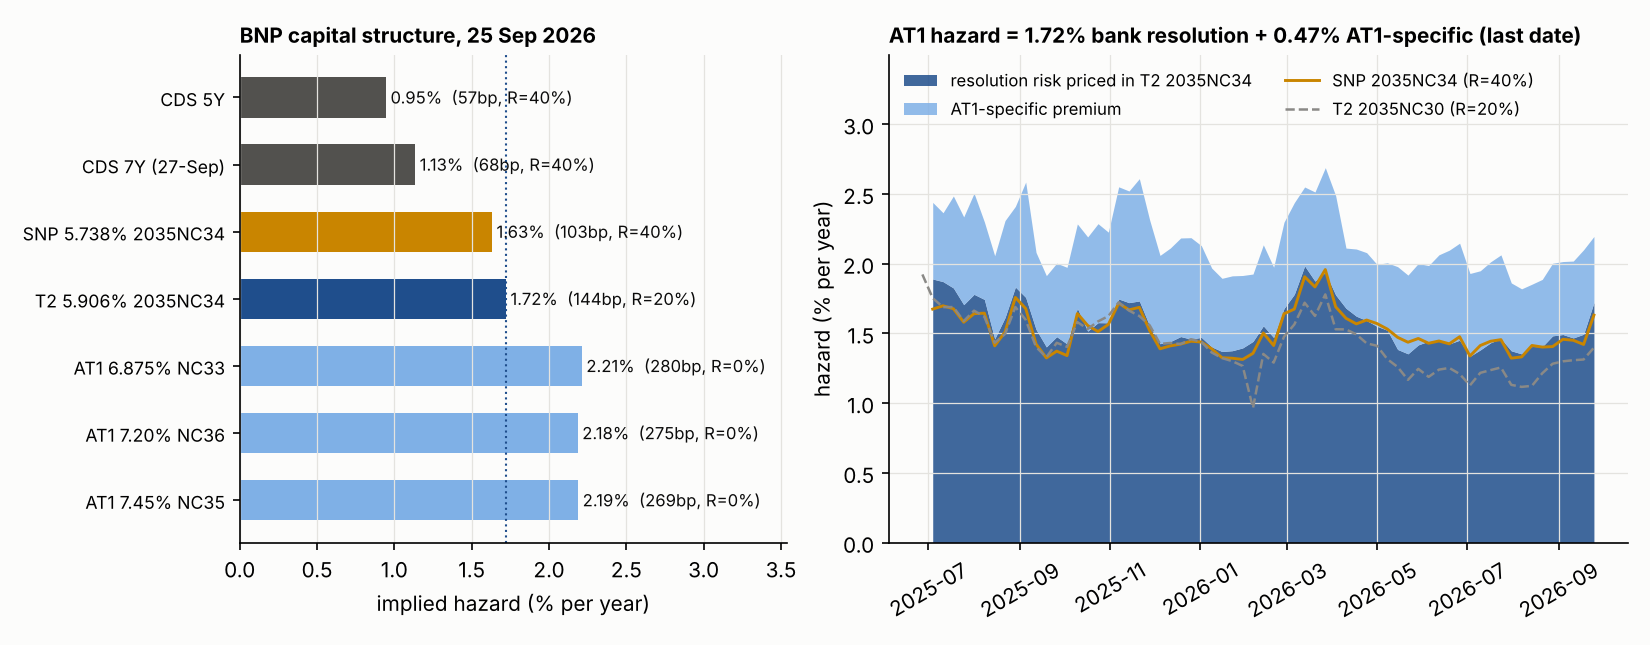
\includegraphics[width=\textwidth]{capital_structure.png}
\caption{Left: implied hazards down BNP's capital structure. Right: the AT1 hazard
(average of the three bonds), weekly, split into the part priced in the Tier~2 2035NC34
and the AT1-specific premium; the SNP and the shorter Tier~2 are shown for comparison.}
\label{fig:capstruct}
\end{figure}

\subsection{What the spread pays for}

Table~\ref{tab:decomp} and Figure~\ref{fig:decomp} give the base attribution of the
yield-to-call spread (order R, S, M, C, E).

\begin{table}[H]
\centering
\begin{tabular}{lccc}
\toprule
bp of yield-to-call spread & 6.875\% NC33 & 7.20\% NC36 & 7.45\% NC35 \\
\midrule
Priced in Tier~2 (resolution) & 181 & 181 & 180 \\
AT1-specific premium & 52 & 49 & 49 \\
MDA coupon cuts & 27 & 31 & 30 \\
Conversion at the trigger & 4 & 4 & 4 \\
Extension & 15 & 9 & 6 \\
\midrule
Total $=$ market & 279 & 274 & 269 \\
\bottomrule
\end{tabular}
\caption{Attribution of the yield-to-call spread, base order. Components are rounded to
sum to the total.}
\label{tab:decomp}
\end{table}

\begin{figure}[H]
\centering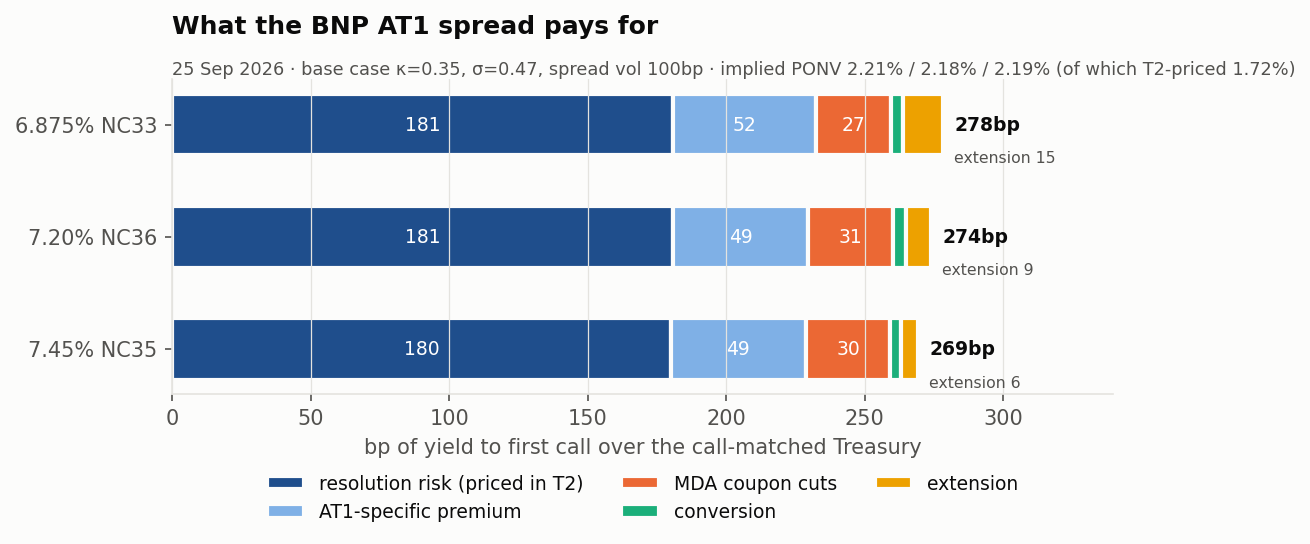
\includegraphics[width=0.88\textwidth]{spread_decomposition.png}
\caption{What the BNP AT1 spread pays for.}
\label{fig:decomp}
\end{figure}

Two-thirds of the spread, about $180$bp, is priced in Tier~2 as well. In the base case
another $50$bp is the premium for being an AT1 rather than a Tier~2: the risk of a write-down
without resolution, the equity-like, perpetual and discretionary profile, and the
instrument's liquidity. This component, unlike the first, depends on the speed of capital
mean reversion (Section~\ref{sec:uncert}). The contract features explain the rest. Expected MDA coupon cuts cost about $30$bp. Conversion
at the trigger, a $1.4$--$1.6\%$ lifetime event at a recovery of about a third, costs
$4$bp. Extension costs $6$--$15$bp and decreases with the reset margin, as it should: the
6.875\% has the lowest margin over today's AT1 spread and pays most for the issuer's option.

The MDA component is an upper bound, for the reasons given in Section~\ref{sec:institutions}:
the model applies the quartile factor to the coupon, while a bank inside its buffer would
cut dividends, buy-backs and variable pay first. Because the total spread is fixed by the
market price, an overstated MDA component is taken from the AT1-specific premium: given
$\kappa$, the $50$bp is a lower bound. Across values of $\kappa$ it is not. Slower capital
rebuilding raises the MDA and extension components and lowers the premium, which is close
to zero at the historical estimate of $\kappa$ (Table~\ref{tab:decompkappa}). What the
market price pins down is their sum with conversion: the $89$--$98$bp that each AT1 pays
over the Tier~2-priced risk.

\subsection{Call and extension}

\begin{table}[H]
\centering
\begin{tabular}{lccc}
\toprule
 & 6.875\% NC33 & 7.20\% NC36 & 7.45\% NC35 \\
\midrule
Reset margin $-$ today's AT1 spread (bp) & $+6$ & $+15$ & $+34$ \\
$\Pr(\text{called at }T_1)$ & 49\% & 52\% & 58\% \\
$\Pr(\text{called at some reset})$ & 97\% & 98\% & 98\% \\
Cost of the issuer's option (points) & 0.78 & 0.59 & 0.37 \\
P\&L if AT1 spreads settle $+50$bp (points) & $-3.3$ & $-3.5$ & $-3.2$ \\
\quad of which from extension (points) & $-1.2$ & $-0.9$ & $-0.7$ \\
\bottomrule
\end{tabular}
\caption{Call and extension. The cost of the option is the price if the call at $T_1$ were
certain minus the model price, at the same hazard. The extension P\&L is the extra loss
relative to a bond whose call at $T_1$ is certain.}
\label{tab:callext}
\end{table}

With a purely economic rule the first call is close to a coin toss, and almost certain at
some later reset. Figure~\ref{fig:calls} shows the probability of a call at the first reset
as a function of the long-run AT1 spread: at $200$bp all three bonds are called about three
times out of four, at $350$bp only a quarter to a third of the time. The low-margin 6.875\%
is always the least likely to be called and is the most negatively convex: if AT1 spreads
settle $50$bp wider, it loses $1.2$ points more than a bond with a certain call. The market
priced exactly this in September 2026: with the ten-year Treasury up 45bp in four weeks,
the 6.875\%'s spread widened by a further 34bp, against 10--12bp for the other two.

\begin{figure}[H]
\centering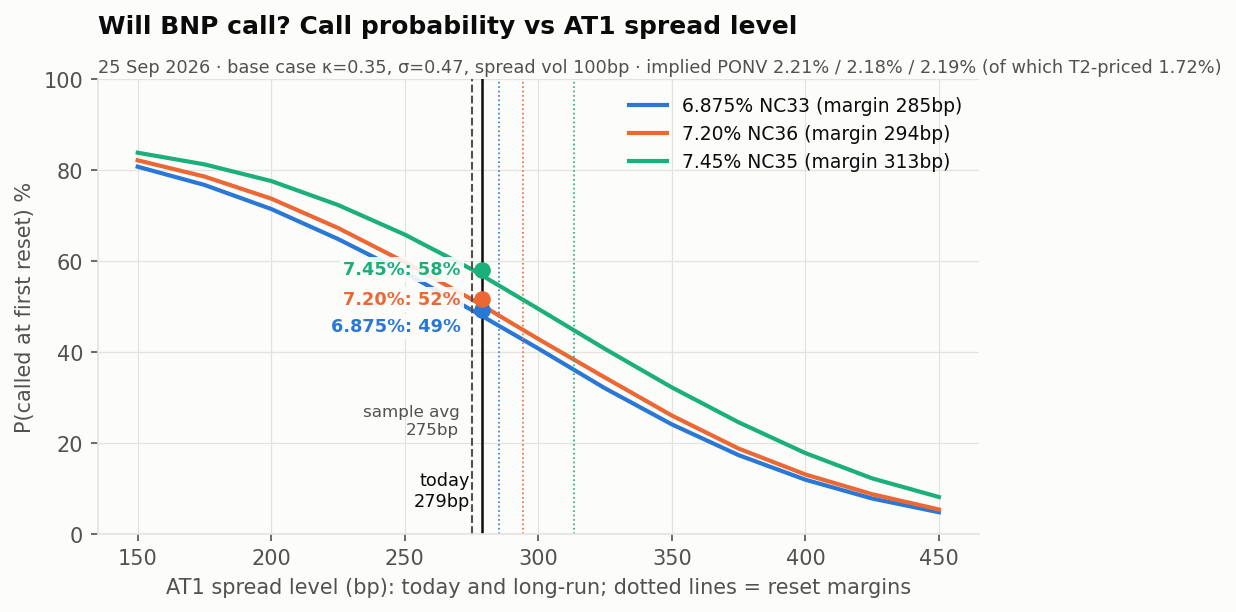
\includegraphics[width=0.8\textwidth]{call_probability.png}
\caption{Probability of a call at the first reset against the AT1 spread level, with
today's and the long-run spread both set to the value on the horizontal axis. Dots: base
case, with today's spread and the long-run level at the sample mean, as in
Table~\ref{tab:callext}.}
\label{fig:calls}
\end{figure}

\subsection{Stress and the capital cliff}

Each scenario of Table~\ref{tab:stress} reprices the bonds on the same random numbers. Rate
shocks move the discount rate and the reset reference; spread shocks move the current and
long-run AT1 spread and scale the hazard with it; capital shocks move today's CET1 ratio.
The two hazard shocks have market counterparts: doubling the Tier~2-priced hazard is roughly
what a doubling of BNP's Tier~2 spread would imply, and it costs three times as much as
doubling the AT1-specific premium.

\begin{table}[H]
\centering
\begin{tabular}{lccc}
\toprule
Clean price change (points) & 6.875\% NC33 & 7.20\% NC36 & 7.45\% NC35 \\
\midrule
Rates $+100$bp & $-5.3$ & $-6.4$ & $-6.1$ \\
Rates $-100$bp & $+5.7$ & $+7.0$ & $+6.7$ \\
CET1 $-2$pp & $-1.5$ & $-1.6$ & $-1.6$ \\
CET1 $-4.2$pp (EBA adverse) & $-9.8$ & $-11.1$ & $-10.4$ \\
AT1 spreads $+200$bp & $-16.4$ & $-16.2$ & $-15.4$ \\
Spreads $+200$bp, rates $-50$bp (March 2023 style) & $-14.5$ & $-13.8$ & $-13.0$ \\
EBA adverse $+$ spreads $+200$bp & $-25.4$ & $-26.6$ & $-25.1$ \\
Tier~2-priced hazard $\times2$ & $-11.9$ & $-13.0$ & $-12.3$ \\
AT1-specific premium $\times2$ & $-3.6$ & $-3.8$ & $-3.6$ \\
\bottomrule
\end{tabular}
\caption{Stress scenarios, base case.}
\label{tab:stress}
\end{table}

\begin{table}[H]
\centering
\begin{tabular}{lcccccc}
\toprule
CET1 level & 13\% (today) & 12\% & 11\% & 10.5\% & 9\% & 7\% \\
\midrule
6.875\% NC33 & 0.6 & 0.8 & 1.7 & 4.4 & 4.6 & 4.6 \\
7.45\% NC35 & 0.6 & 0.8 & 1.9 & 4.8 & 4.8 & 4.8 \\
\bottomrule
\end{tabular}
\caption{Capital delta: price points per $+1$pp of CET1, by CET1 level (finite differences
on a $0.5$pp grid).}
\label{tab:delta}
\end{table}

\begin{figure}[H]
\centering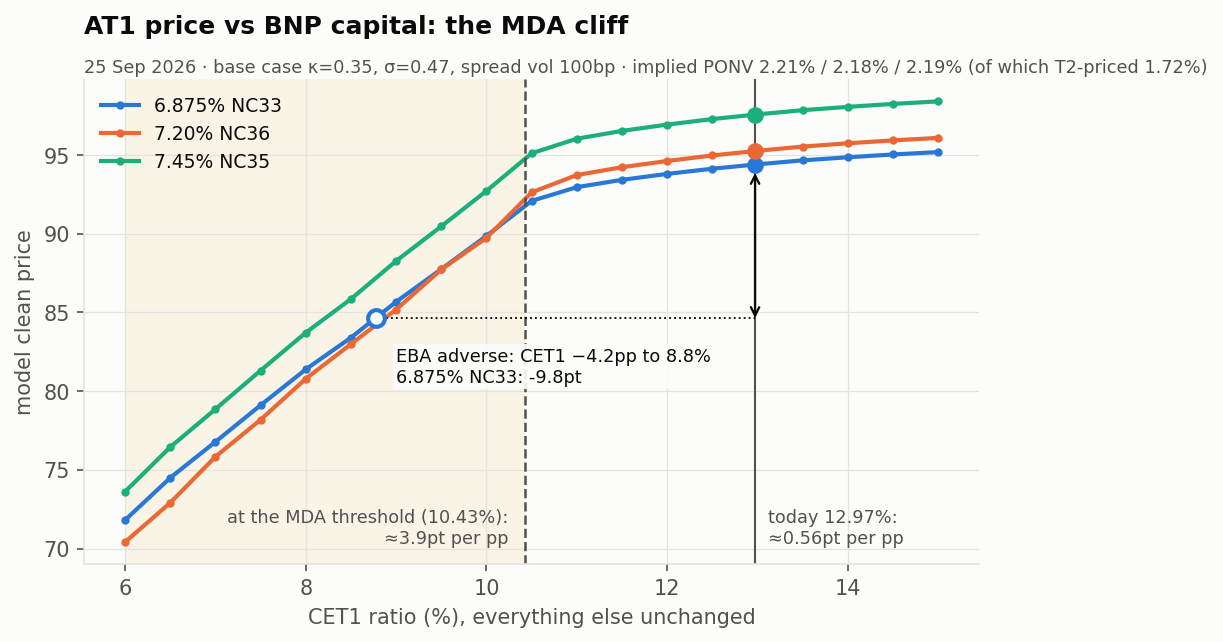
\includegraphics[width=0.8\textwidth]{price_vs_cet1.png}
\caption{Model price against today's CET1 ratio, everything else unchanged.}
\label{fig:cliff}
\end{figure}

Table~\ref{tab:delta} and Figure~\ref{fig:cliff} show the capital cliff. At today's ratio
the price moves by about $0.6$ points per point of CET1; within a point of the MDA threshold
the sensitivity rises to $4$--$5$ points. Crossing the threshold switches on three mechanisms
at once: coupons are cut by \eqref{eq:mda}, the call is blocked by \eqref{eq:call}, and the
hazard rises through \eqref{eq:seff}--\eqref{eq:hazard}. Because the O-SII step-ups raise the
threshold by 50bp by 2028, a capital loss of about half the EBA adverse depletion moves the
bonds from the flat part of the curve onto the cliff. The relevant risk measure for these
bonds is the distance to the MDA threshold, not the distance to the trigger.

\subsection{How much can we trust the capital parameters?}\label{sec:uncert}

Table~\ref{tab:kappa} reports the headline results, averaged across the three bonds, at the
two ends of the bootstrap interval for $\kappa$, at the maximum likelihood estimate and in the
base case. Each column recalibrates the implied hazards of the AT1s and, on the same paths,
the hazard of the Tier~2 anchor.

\begin{table}[H]
\centering
\begin{tabular}{lcccc}
\toprule
 & $\kappa=0.06$ & $\kappa=0.165$ & $\kappa=0.35$ & $\kappa=0.48$ \\
 & (5\%) & (MLE) & (base) & (95\%) \\
\midrule
Half-life of a capital shock (years) & 11.0 & 4.2 & 2.0 & 1.5 \\
Implied hazard (\%/yr) & 0.66 & 1.64 & 2.20 & 2.33 \\
\quad priced in Tier~2, $\lres$ (\%/yr) & 1.61 & 1.67 & 1.72 & 1.74 \\
\quad AT1-specific, $\lspec$ (\%/yr) & $-0.95$ & $-0.03$ & 0.47 & 0.59 \\
\quad Tier~2 share of the AT1 hazard & 244\% & 102\% & 78\% & 75\% \\
MDA coupon cost (points) & 14.5 & 6.3 & 2.5 & 1.7 \\
Capital delta at the MDA threshold (points/pp) & 13.7 & 8.8 & 4.2 & 2.8 \\
EBA adverse shock (points) & $-37.7$ & $-21.4$ & $-10.5$ & $-7.3$ \\
Cross-bond dispersion $D$ (bp) & 7.8 & 4.2 & 2.6 & 2.3 \\
\quad in price points & 0.6 & 0.3 & 0.2 & 0.2 \\
Log-likelihood relative to MLE & $-0.5$ & 0 & $-1.5$ & $-4.1$ \\
\bottomrule
\end{tabular}
\caption{Sensitivity to the speed of capital mean reversion (average of the three bonds).
$\lres$ is re-implied from the Tier~2 2035NC34 on the paths of each column. The capital
delta at the threshold is the central difference over $\pm0.25$pp.}
\label{tab:kappa}
\end{table}

\begin{figure}[H]
\centering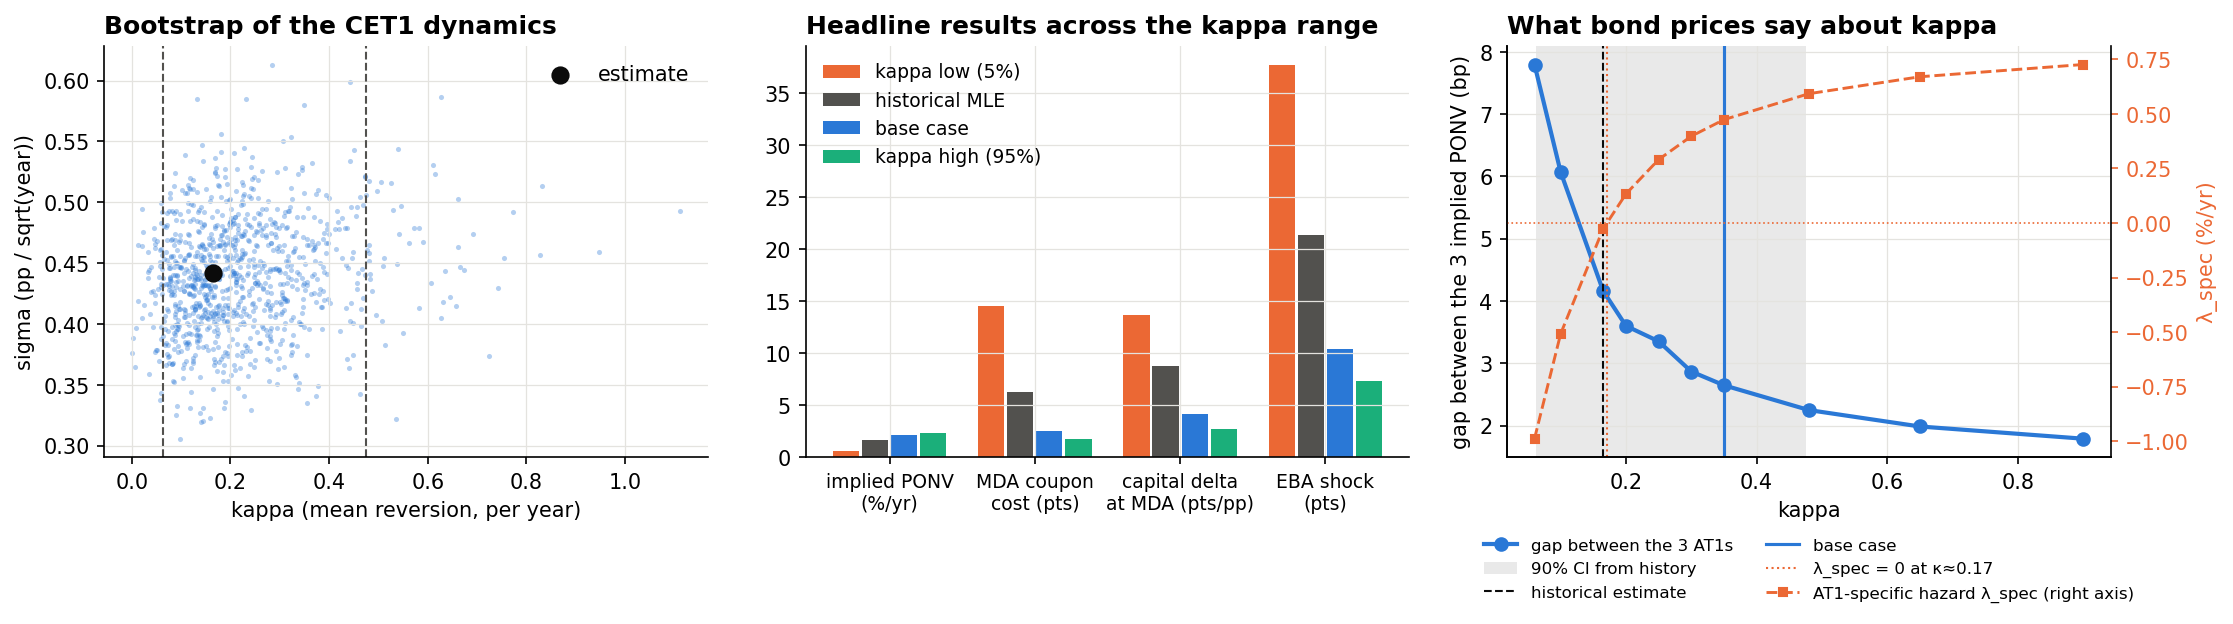
\includegraphics[width=\textwidth]{parameter_uncertainty.png}
\caption{Left: bootstrap of $(\kappa,\sigma)$. Centre: headline results across the
$\kappa$ range. Right: cross-bond dispersion of the implied hazard against $\kappa$ (left
axis) and the AT1-specific hazard $\lspec$ (right axis); the dotted line marks
$\lspec=0$.}
\label{fig:uncert}
\end{figure}

\paragraph{What prices add.} History and prices pull in opposite directions. The three
bonds are more consistent with fast capital rebuilding: the dispersion falls from $7.8$bp at
$\kappa=0.06$ to $2.3$bp at $0.48$ and then flattens. In price terms this is $0.6$ against
$0.2$ points, around the bid--offer, so the evidence is a lean, not an identification. The
history disfavours values much above $0.35$: the likelihood ratio statistic is $3.1$ at
$0.35$ and $8.1$ at $0.48$, and crosses the $5\%$ critical value of $3.84$ at about
$\kappa=0.37$.

\paragraph{What the Tier~2 adds.} The Tier~2 anchor gives a sharper restriction than the
cross-section of AT1s. Re-solved on the paths of each $\kappa$, the hazard priced in Tier~2
barely moves, from $1.61\%$ a year at $\kappa=0.06$ to $1.74\%$ at $\kappa=0.48$, so the
sensitivity to the capital dynamics falls almost entirely on the AT1-specific hazard. That
hazard is negative below $\kappa\approx0.17$: when capital is slow to rebuild, the model
attributes so much of the AT1's discount to expected MDA coupon cuts that the AT1 would be
priced as less risky than BNP's own Tier~2, which the creditor hierarchy rules out.
Requiring $\lspec\ge0$ excludes the lower half of the bootstrap interval and places the
bound at $\kappa=0.171$ for the average of the three bonds ($0.175$ for each bond
separately), a value that the history cannot distinguish from its maximum likelihood
estimate. Together with the likelihood, the admissible range is $\kappa\in[0.17,0.37]$, a
half-life of capital shocks between $1.9$ and $4.1$ years, over which $\lspec$ runs from zero
to about $0.49\%$ a year. The base case $\kappa=0.35$ lies in the upper part of this range,
where the cross-section of AT1s also points, and is consistent with BNP's active capital
management.

Table~\ref{tab:decompkappa} repeats the attribution of the spread at the two ends of the
admissible range, with $\sigma$, the AT1 hazards and the Tier~2 hazard re-solved for each
$\kappa$. The component priced in Tier~2 moves by less than half a basis point, and so does
the total that the AT1 pays over it. What moves is the split of that total. At
$\kappa=0.17$ the AT1-specific premium vanishes and its place is taken by expected coupon
cuts and by extension: with slow capital rebuilding, CET1 is more often below the MDA
threshold on a reset date, so the call is blocked more often and extension costs three
times as much as in the base case. Between $\kappa=0.35$ and $\kappa=0.37$ the attribution
hardly changes.

\begin{table}[H]
\centering
\begin{tabular}{lccc}
\toprule
bp of yield-to-call spread & $\kappa=0.171$ & $\kappa=0.35$ (base) & $\kappa=0.37$ \\
\midrule
Priced in Tier~2 (resolution) & 180.1 & 180.5 & 180.5 \\
AT1-specific premium & 1.0 & 49.8 & 52.3 \\
MDA coupon cuts & 52.0 & 29.4 & 27.9 \\
Conversion at the trigger & 6.7 & 4.3 & 4.1 \\
Extension & 34.0 & 10.0 & 9.1 \\
\midrule
AT1 over Tier~2 (premium and contract features) & 93.8 & 93.4 & 93.4 \\
Total $=$ market & 273.9 & 273.9 & 273.9 \\
\bottomrule
\end{tabular}
\caption{Attribution of the yield-to-call spread (base order, average of the three bonds)
at the ends of the range of $\kappa$ admitted by the CET1 history and the Tier~2
restriction, and in the base case. Each column re-solves $\sigma$, the AT1 hazards and the
Tier~2 hazard.}
\label{tab:decompkappa}
\end{table}

Two caveats qualify the bound. It is conditional on the stylised MDA rule: because
\eqref{eq:mda} overstates the expected coupon loss, and most so when capital is slow to
rebuild, the true bound lies below $0.17$. And $\lspec=0$ is the weakest restriction the
hierarchy imposes; any positive liquidity or equity premium on the AT1 would raise it.

\paragraph{Where the uncertainty sits.} With a slower mean reversion a capital shock lasts
longer, so more paths spend time inside the buffer: the MDA cost and the capital delta rise
and, since the total is fixed by the price, the implied hazard falls. Figure~\ref{fig:cliffunc}
re-calibrates each curve to today's price of the 6.875\%. All four agree at today's
$13\%$ CET1, and diverge only as capital falls: at the MDA threshold the price ranges from
$76$ ($\kappa=0.06$) to $93$ ($\kappa=0.48$), and at $6\%$ CET1 from $36$ to $77$. Bond prices
identify the level of risk today, not the shape of the cliff. What is robust across the
interval is the hazard priced in Tier~2, the ordering of the three bonds, the extension
ranking and the steepening of the capital delta near the threshold. The level of the
capital stress and the split of the AT1's excess over the Tier~2 among the AT1-specific
premium, the MDA component and extension are not; the Tier~2 restriction narrows their
range but does not remove it.

\begin{figure}[H]
\centering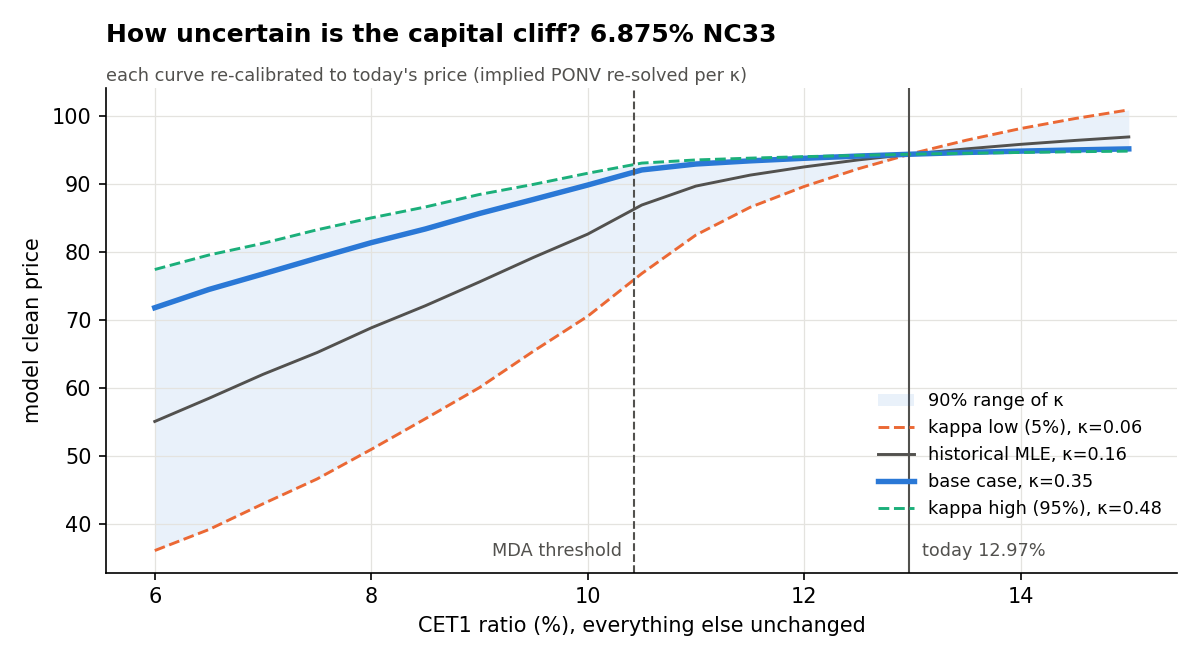
\includegraphics[width=0.8\textwidth]{capital_cliff_uncertainty.png}
\caption{Price of the 6.875\% NC33 against CET1 for four values of $\kappa$, each
re-calibrated to today's price. Shaded: $90\%$ bootstrap range of $\kappa$.}
\label{fig:cliffunc}
\end{figure}